\section{Empty run through}
I thought it would be good to try and categorise the static pressure losses from the flow through the tank with no sand and no piston. Unfortunately, this immediately presented some problems. Results of this test are seen below.
\begin{figure}[htbp]
    \centering

    \begin{minipage}{0.45\textwidth}
        \centering
        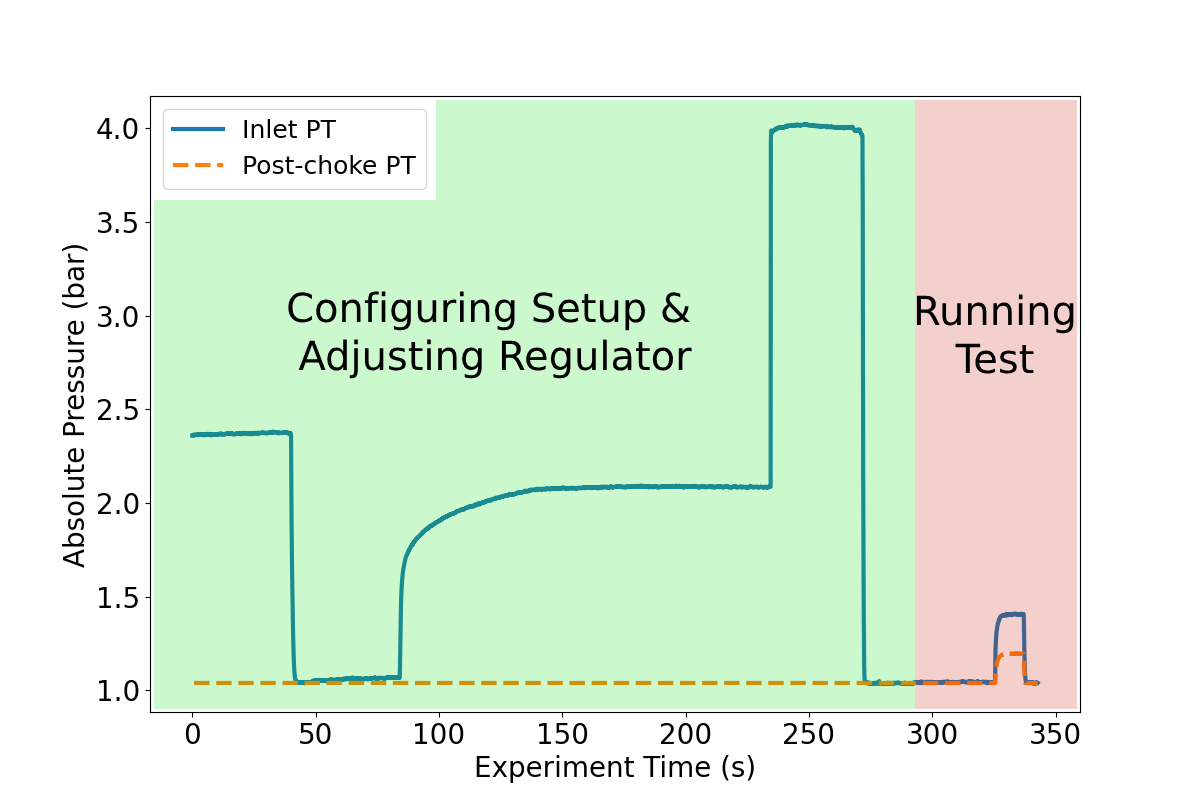
\includegraphics[width=\textwidth]{../report_assets/3_bar_static_full.png}
        \caption{pressure readings full.}\label{fig:static-pressure-drop-3bar_full}
    \end{minipage}
    \hfill
    \begin{minipage}{0.45\textwidth}
        \centering
        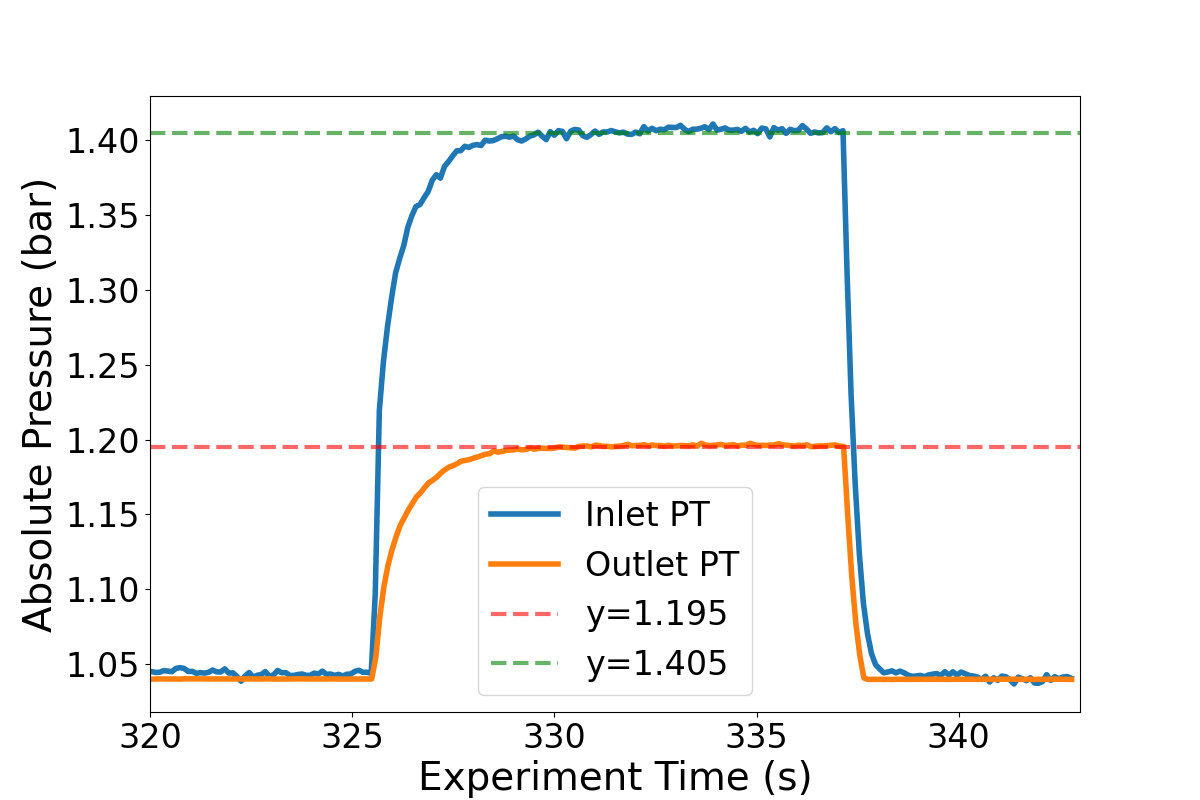
\includegraphics[width=\textwidth]{../report_assets/3_bar_static.png}
        \caption{pressure readings of 3bar gauge.}\label{fig:static-pressure-drop-3bar}
    \end{minipage}
    \begin{minipage}{0.45\textwidth}
        \centering
        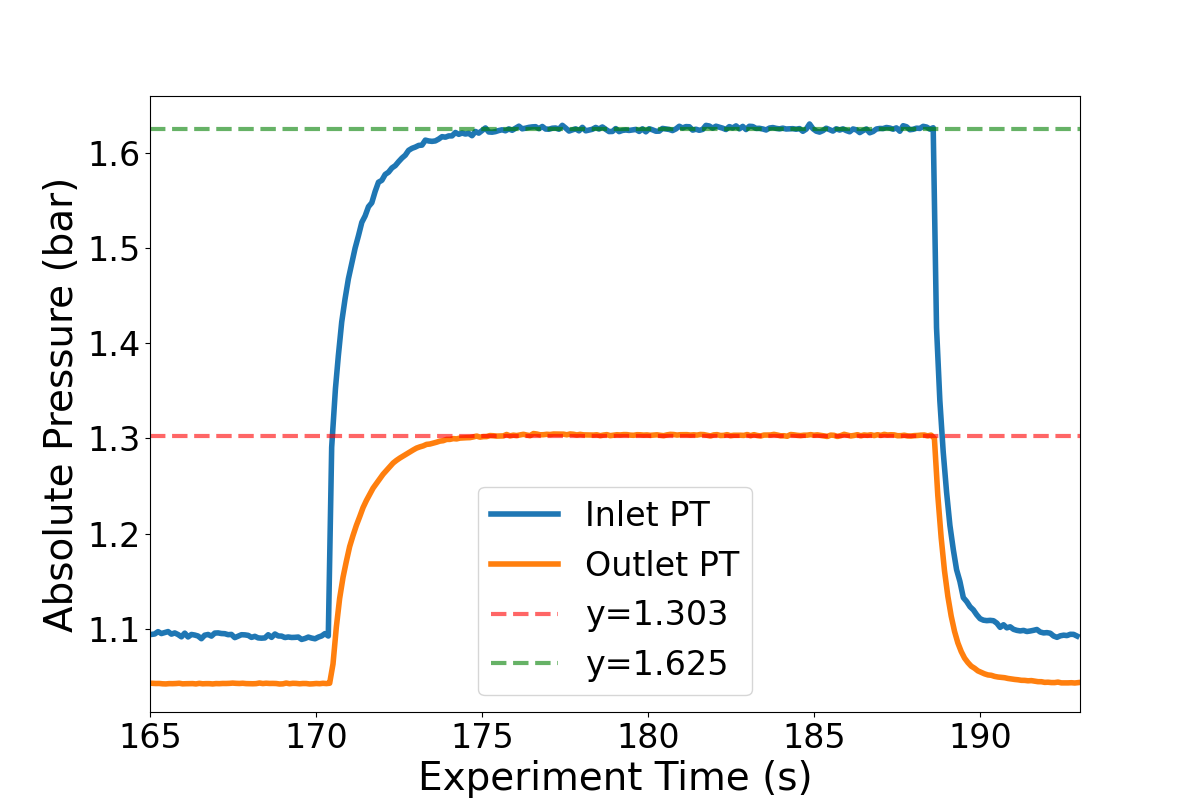
\includegraphics[width=\textwidth]{../report_assets/4_bar_static.png}
        \caption{pressure readings of 4bar gauge.}\label{fig:static-pressure-drop-4bar}
    \end{minipage}
    \hfill
    \begin{minipage}{0.45\textwidth}
        \centering
        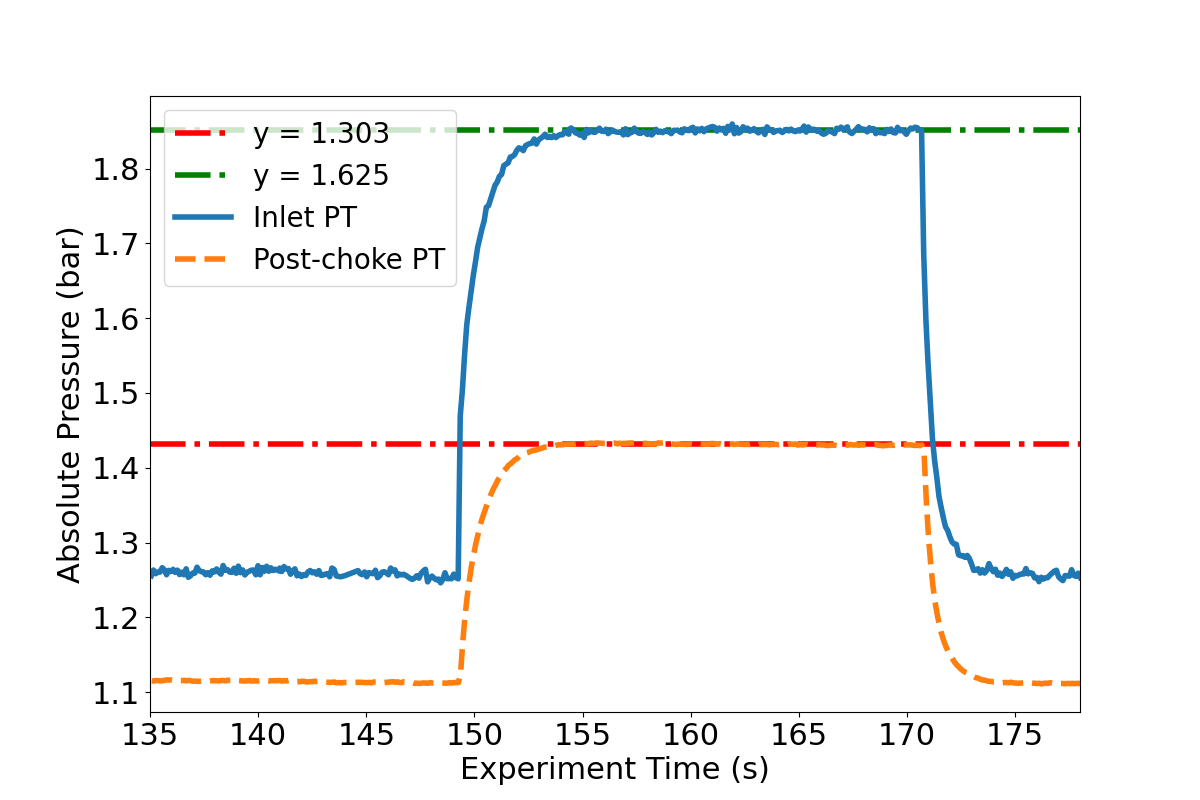
\includegraphics[width=\textwidth]{../report_assets/5_bar_static.png}
        \caption{pressure readings of 5bar gauge.}\label{fig:static-pressure-drop-5bar}
    \end{minipage}


\end{figure}
One thing of note is that the pressure transducer readings seem to deviate from atmospheric in fig 3 and 4. This is due to the solenoid valve leaking slightly allowing some air to pass through not miscalibration, yap about in appendix.

As seen in figure 1, the regulator was able to control the static pressure to 3 bar gauge when the system was closed. When the system was opened this static pressure dropped to 0.4 gauge. Even accounting for the dynamic pressure and assuming the flow was mach 1 through the 4mm nylon tube, this would put total pressure at roughly 1bar gauge not 3bar initially set.
\section{first test}
\begin{figure}[htbp]
    \centering

    \begin{minipage}{0.45\textwidth}
        \centering
        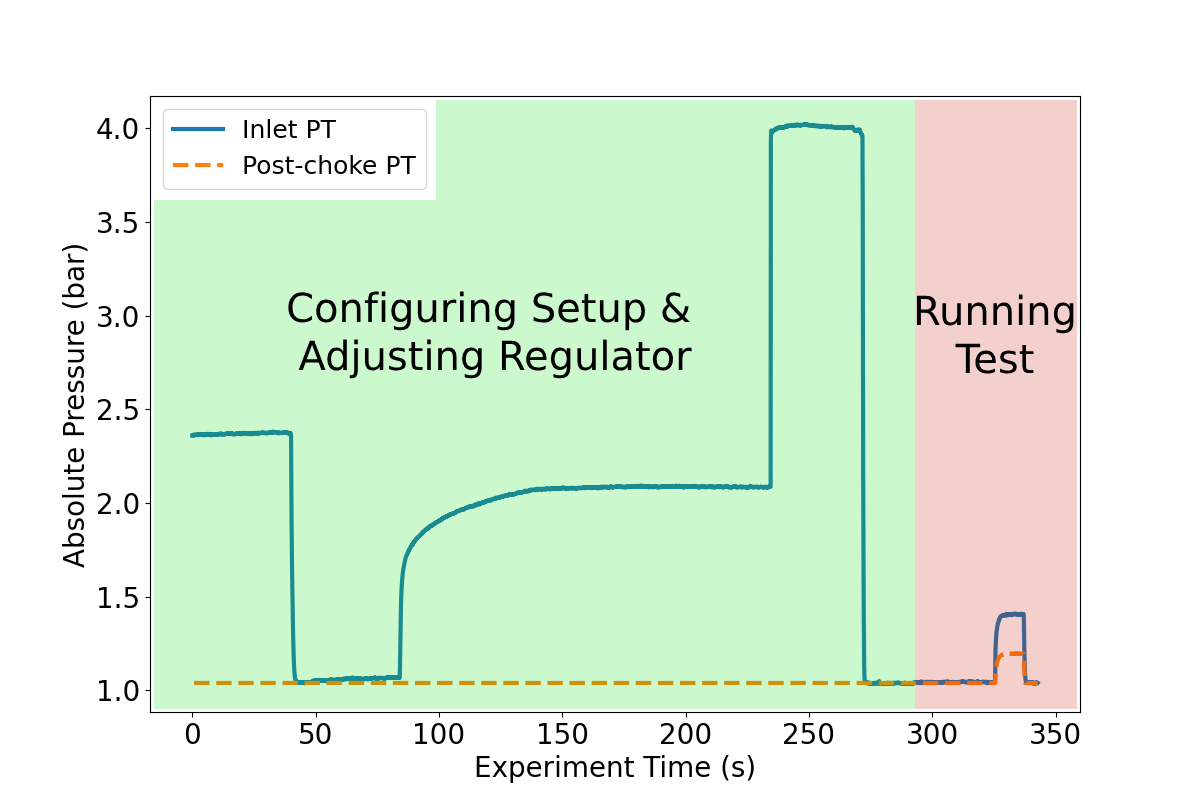
\includegraphics[width=\textwidth]{../report_assets/3_bar_static_full.png}
        \caption{pressure readings full.}\label{fig:static-pressure-drop-3bar_full}
    \end{minipage}
    \hfill
    \begin{minipage}{0.45\textwidth}
        \centering
        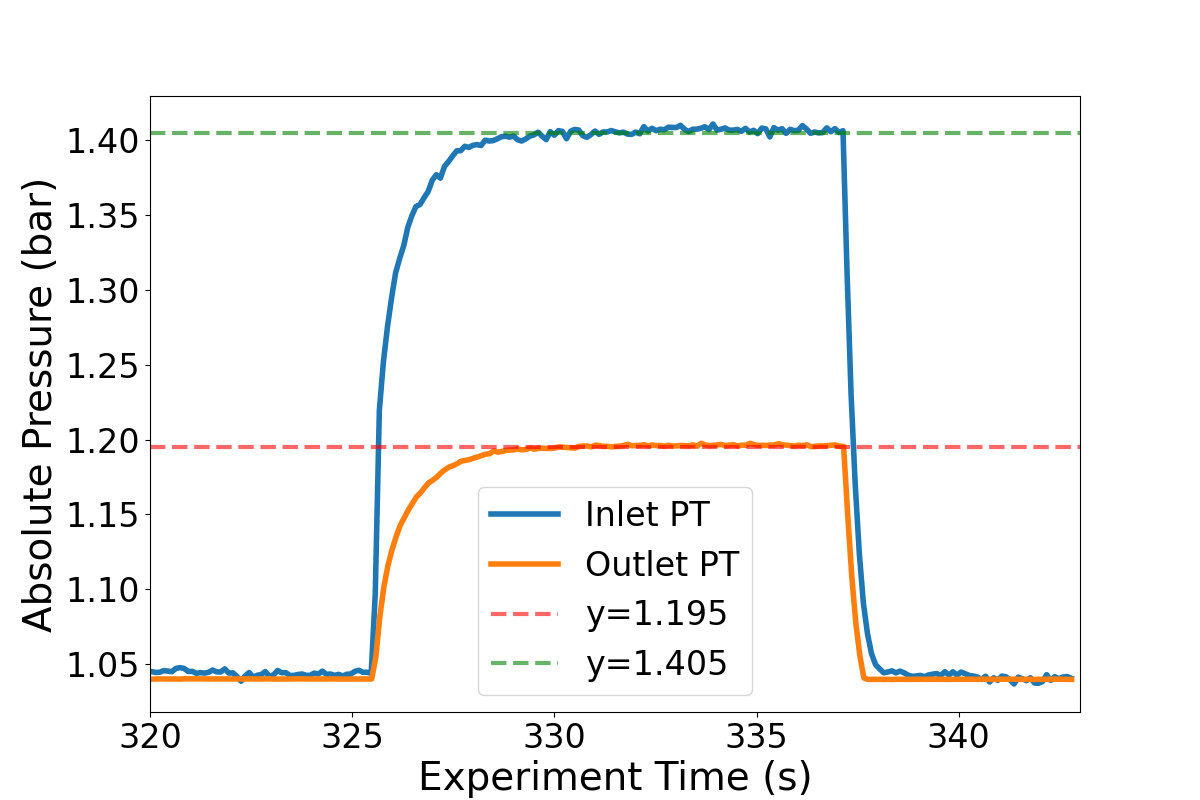
\includegraphics[width=\textwidth]{../report_assets/3_bar_static.png}
        \caption{pressure readings of 3bar gauge.}\label{fig:static-pressure-drop-3bar}
    \end{minipage}

\end{figure}
highlighted the issue of the piston locking up,
force required to compact the sand to the outlet
sand only at the top moved
no fluidisation behaviours observed, maybe higher pressures required after all
chokepoint blocked sand and prevented flow into cyclone seperator
\section{Piston velocity - mass flow rate relation}
didnt really work. idk why but it should have
\section{Piston design}
due to granular material being bigger than typical, often gets stucka round the piston and causes it to lock up

redesign
modelling the piston as a circle and the sand as a fluid. 
P = rho * h * g
P = 1529 * (74mm - y) * 9.81~= 15000* (74mm - y)
\begin{equation}
    \int_{-0.037}^{0.037}\!\int_{0}^{0.037+\sqrt{0.037^2 - x^2}}15000\,(0.074 - y)\,\mathrm{d}y\,\mathrm{d}x
    \;-\;
    \int_{-0.037}^{0.037}\!\int_{0}^{0.037-\sqrt{0.037^2 - x^2}}15000\,(0.074 - y)\,\mathrm{d}y\,\mathrm{d}x.
\end{equation}

% \begin{equation}
%     15000\int_{-0.037}^{0.037}\Bigl(0.037^2 + \frac{x^2}{2} + 0.037\sqrt{0.037^2 - x^2}\Bigr)\,\mathrm{d}x = 0.302369.
% \end{equation}
% \begin{equation}
%     15000\int_{-0.037}^{0.037}\Bigl(0.037^2 + \frac{x^2}{2} - 0.037\sqrt{0.037^2 - x^2}\Bigr)\,\mathrm{d}x = 0.302369.
% \end{equation}
\begin{equation}
    15000\int_{-0.037}^{0.037}\Bigl(0.037^2 + \tfrac{x^2}{2} + 0.037\sqrt{0.037^2 - x^2}\Bigr)\,\mathrm{d}x
    \;-\;
    15000\int_{-0.037}^{0.037}\Bigl(0.037^2 + \tfrac{x^2}{2} - 0.037\sqrt{0.037^2 - x^2}\Bigr)\,\mathrm{d}x
\end{equation}
\begin{equation}
    15000\int_{-0.037}^{0.037}\Bigl(0.074\sqrt{0.037^2 - x^2}\Bigr)\,\mathrm{d}x = 2.38697N
\end{equation}

555.001308106 Pa average pressure differential across the two piston faces to get this force required to compact the sand

deltaP for fluidising bed is $h*(rho_s - rho_a)*9.81$ which is 0.2 1527 10 = 300pa


sand drops static pressure only. Therefore probably need to make the piston drop about half a bar of static pressure aswell
this is easily testable in the setup

need to think about friction when testing for a certain dp across the faces

need to think about the sand when designing for the geometry so it doesnt get stucka

might run into the inherent cocking issue since pressure from sand is concentrated at the bottom

static pressure losses from the tank and set up alone

3 bar (gauge) total goes to 1.405bar static and 1.195bar static = loss of 0.210bar static
4 bar (gauge) total goes to 1.625bar static and 1.303bar static = loss of 0.322bar static
5 bar (gauge) total goes to 1.852bar static and 1.432bar static = loss of 0.420bar static

static pressure losses from the tank + piston

3 bar (gauge) total goes to 1.425bar static and 1.209bar static = loss of 0.216bar static
4 bar (gauge) total goes to 1.628bar static and 1.304bar static = loss of 0.324bar static
5 bar (gauge) total goes to 1.831bar static and 1.431bar static = loss of 0.400bar static

static pressure losses from the tank + new piston

3 bar (gauge) total goes to 1.423bar static and 1.205bar static = loss of 0.218bar static
4 bar (gauge) total goes to 1.645bar static and 1.311bar static = loss of 0.334bar static
5 bar (gauge) total goes to 1.850bar static and 1.450bar static = loss of 0.400bar static

